\documentclass[SE,authoryear,toc]{lsstdoc}
\input{meta}

% Package imports go here.
\usepackage{graphicx} 
\usepackage{amsmath} 
\usepackage{amssymb}
\usepackage{mathtools}
\usepackage{amsmath,bm}

% Local commands go here.
\renewcommand{\v}[1]{\mathbf{#1}}
\newcommand{\plus}{\scalebox{0.6}{$+$}}
\newcommand{\tr}{\scalebox{0.6}{$\top$}}
\DeclarePairedDelimiter{\norm}{\lVert}{\rVert}

%If you want glossaries
%\input{aglossary.tex}
%\makeglossaries

\title{Notes on Optical Feedback Controller}

% This can write metadata into the PDF.
% Update keywords and author information as necessary.
\hypersetup{
    pdftitle={Notes on Optical Feedback Controller},
    pdfauthor={Guillem Megias Homar},
    pdfkeywords={},
    colorlinks=true,
    allcolors=blue
}

% Optional subtitle
% \setDocSubtitle{A subtitle}

\author{%
Guillem Megias Homar
}

\setDocRef{SITCOMTN-129}
\setDocUpstreamLocation{\url{https://github.com/lsst-sitcom/sitcomtn-129}}

\date{\vcsDate}

% Optional: name of the document's curator
% \setDocCurator{The Curator of this Document}

\setDocAbstract{%
The Rubin Observatory active optics system (AOS) uses the optical feedback controller (OFC) to estimate the degree of freedom corrections of the telescope from wavefront error estimates obtained with WEP from out-of-focus images of stars. This note describes the theory behind different control approaches and derives the equations used by OFC.
}

% Change history defined here.
% Order: oldest first.
% Fields: VERSION, DATE, DESCRIPTION, OWNER NAME.
% See LPM-51 for version number policy.
\setDocChangeRecord{%
  \addtohist{1}{2024-06-06}{Initial version.}{Guillem Megias Homar}
}


\begin{document}

% Create the title page.
% \maketitle
\mkshorttitle
% Frequently for a technote we do not want a title page  uncomment this to remove the title page and changelog.
% use \mkshorttitle to remove the extra pages


\subsection*{Motivation}
The LSST active optics system (AOS) uses wavefront information to correct for errors in the rigid body displacement and rotation of M2 and the camera relative to M1M3 and for bending deformations of both M2 and M1M3; these degrees of freedom will collectively be referred to the optical state of the telescope. A look-up table (LUT) will correct for most of the gravity-induced motion; only the residual due to thermal variations, dome seeing or errors in the gravity look-up table needs to be corrected by AOS. Wavefront information is available from four field points and used to correct motion every 30 seconds. 

To determine how to adjust the optical state, so that the wavefront error is minimized, we use the wavefront information to estimate the optical state of the system and derive from there what are the corrections, in the basis of the degrees of freedom, that need to be applied.

Given that we are able to set the degrees of freedom values, one may wonder why we need to estimate them from the wavefront sensing if we have control over them. Thermal variations, gravitational errors, and dome-seeing affect the optical aberrations of the telescope and, therefore, the optical state. The fact that we express the optical state on the basis of the degrees of freedom doesn't mean we are estimating the state of the degrees of freedom at the actuator-level, which we know exactly, but rather the optical state of the system which is due to the actuator-level motions and the optical aberration effects. 

\subsection*{Preliminaires}
The vector of wavefront measurements $\symbf{y} \in \mathbb{R}^n$ and the optical state vector  $\symbf{x} \in \mathbb{R}^m$ are related through the sensitivity matrix $\v{A} \in \mathbb{R}^{n \times m}$ as $\symbf{y} = \v{A} \symbf{x}$. 

We will consider the vector of wavefront measurements $\symbf{y}$ to be a 19-dimensional vector with Zernike coefficients from $Z_4$ to $Z_{22}$. However, we could consider the $\symbf{y}$ to be the 19-Zernike vector at different Gaussian quadrature points, in which case $\symbf{y} \in \mathbb{R}^{p \times n}$ where $p$ are the number of quadrature points. If that were the case, then the sensitivity matrix would be $\v{A} \in \mathbb{R}^{p \times n \times m}$. We could unravel the vectors and end up with an equivalent description to the original one. Therefore, without loss of generality, we will keep the dimensions of $\symbf{y}$ to be $n$ for this summary.

The optical state vector  $\\symbf{x}$ is a 50-dimensional vetor corresponding to the $50$ degrees of freedom of our system, which include by order, the rigid-body motion hexapod degrees of freedom for M2 ($dz_{M2}$, $dx_{M2}$, $dy_{M2}$, $Rx_{M2}$, $Ry_{M2}$) and for the Camera hexapod ($dz_{Cam}$, $dx_{Cam}$, $dy_{Cam}$, $Rx_{Cam}$, $Ry_{Cam}$), the 20 bending modes of M1M3, and the 20 bending modes of M2. 

We will denote the vector of corrections that we apply to the system as $\\symbf{u} \in \mathbb{R}^n$. These corrections are also on the basis of the degrees of freedom.

Finally, we will assume the following description of the optical state at time-step $k + 1$ holds, 
\begin{equation}\label{eq3}
    \\symbf{x}_{k + 1} = \\symbf{x}_{k} + \\symbf{u} + \\symbf{\delta}_{k}
\end{equation}
where $\\symbf{\delta}_{k}$ is the average deviation introduced between time-step due to uncontrolled effects.

\subsection*{Optical state estimation}
The simplest way to estimate the optical state from the wavefront error measurements --which corresponds to the way we currently do it in \texttt{ts\_ofc}-- is using the Moore-Penrose pseudoinverse ($\v{A}^{\plus}$), which is derived as follows,
\begin{equation*}
     \v{A}\\symbf{x} = \\symbf{y}
\end{equation*}
\begin{equation*}
     \v{A}^{\tr}\v{A}\\symbf{x} = \v{A}^{\tr}\\symbf{y}
\end{equation*}
\begin{equation*}
    \hat{\\symbf{x}} = (\v{A}^{\tr} \v{A})^{-1}\v{A}^{\tr}\\symbf{y} = \v{A}^{\plus}\\symbf{y}
\end{equation*}

Notably, the sensitivity matrix is a highly-degenerate matrix which has a set of singular vectors with very small singular values. In Figure \ref{fig1} we plot the singular values for the Sensitivity matrix calculated on 35 Gaussian Quadrature points in the corner wavefront sensors. 

\begin{figure}[h!]
    \centering
    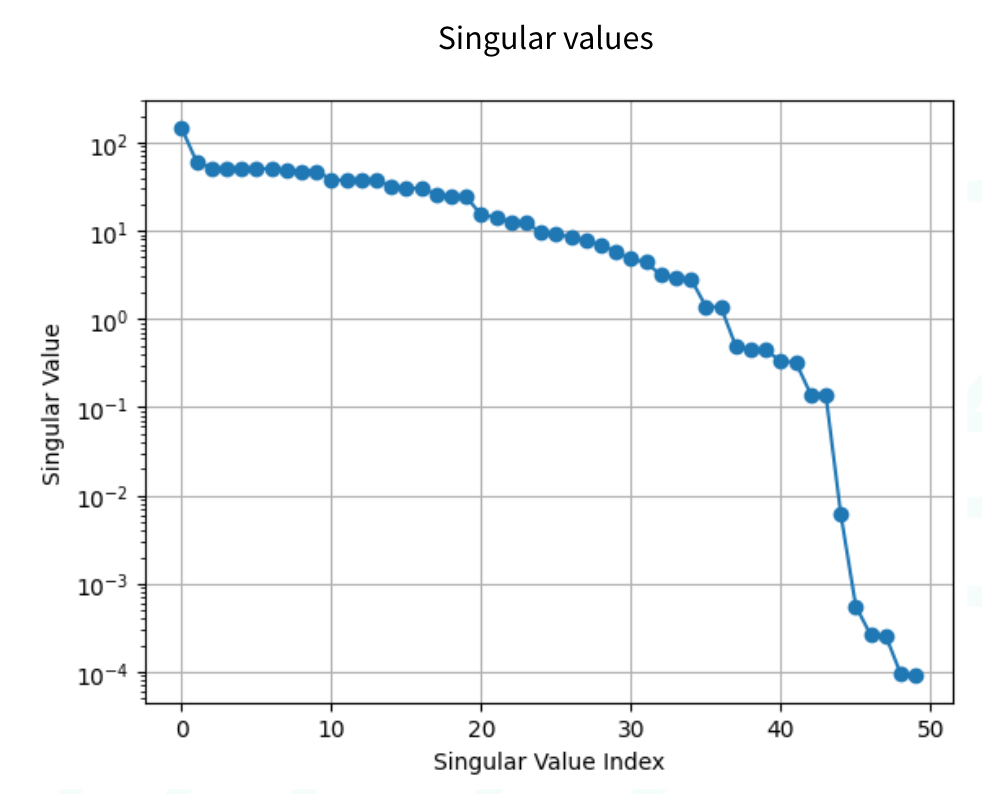
\includegraphics[scale = 0.5]{figures/singular_values.png}
    \caption{Singular values derived from the original sensitivity matrix at the 35 Gaussian Quadrature points of the four wavefront sensors.}
    \label{fig1}
\end{figure}

The importance of the degeneracy on our optical feedback control comes into play at multiple levels. The first one is the pseudo-inverse. In fact, instead of doing this matrix multiplication above, the pseudo-inverse $\v{A}^{\plus}$ is computed \textit{de facto} using the Singular Value Decomposition (SVD) of $\v{A}$.
\begin{equation}
     \hat{\\symbf{x}} = \v{A}^{\plus}\\symbf{y} = \v{V} \v{\Sigma}^{-1} \v{U^{\tr}}\\symbf{y}
\end{equation}
The singular vectors from the sensitivity matrix, therefore play a crucial role in our state estimate. Let us rewrite the state estimate based on the real optical state $\\symbf{x}$,
\begin{equation}
     \hat{\\symbf{x}} = \v{A}^{\plus}\\symbf{y} = \v{A}^{\plus}\v{A}\\symbf{x} = \v{V}\v{\Sigma}^{-1} \v{U^{\tr}}\v{U} \v{\Sigma} \v{V^{\tr}}\\symbf{x} =  \v{V}\v{V^{\tr}}\\symbf{x}
\end{equation}

Since $\v{A}$ is nearly-degenerate, it doesn't have full column rank, and therefore $\v{V}\v{V^{\tr}} \neq \mathbb{I}$. In this case, we can interpret the pseudo-inverse estimate $\hat{\\symbf{x}}$ as the orthogonal projection of $\\symbf{x}$ onto the row space of $\v{A}$. 


\subsubsection*{Noisy measurements}
Let us now depart from the ideal world of physics and delve into reality. In this case, the problem formulation can be rewritten introducing noise to our measurements as,
\begin{equation}
    \\symbf{y}_{noisy} = \v{A} \\symbf{x} + \\symbf{w}
\end{equation}

The first step is to study what the error of our previous pseudo-inverse estimate will look like, that is, what is our \textit{reconstruction} error. The noisy estimate, in this case, would be, 
\begin{equation}
    \hat{\\symbf{x}}_{noisy} = \v{A}^{\plus}\v{A}\\symbf{x} +\v{A}^{\plus}\\symbf{w} 
\end{equation}

So the reconstruction error would be, 
\begin{equation}
    \norm{\hat{\\symbf{x}}_{noisy} - \hat{\\symbf{x}}}_2^2 = \norm{\v{A}^{\plus}\\symbf{w} }_2^2 = \norm{\v{V}\v{\Sigma}^{-1}\v{U}^{\tr}\\symbf{w} }_2^2
\end{equation}

Where we used the SVD of $\v{A}$. Now, let us show that for any vector $\\symbf{z} \in \mathbb{R}^n$, 
\begin{equation}
    \norm{\v{V}\\symbf{z}}_2^2 = \\symbf{z}^{\tr}\v{V}^{\tr}\v{V}\\symbf{z} = \\symbf{z}^{\tr}\\symbf{z} =  \norm{\\symbf{z}}_2^2
\end{equation}
where we used the fact that the right-singular vector matrix derived from SVD is such that, $\v{V}^{\tr}\v{V} = \mathbb{I}$

Now our reconstruction error can be rewritten as, 
\begin{equation}
    \norm{\hat{\\symbf{x}}_{noisy} - \hat{\\symbf{x}}}_2^2 = \norm{\v{\Sigma}^{-1}\v{U}^{\tr}\\symbf{w} }_2^2
\end{equation}

At this point, let us suppose for just a minute that the noise is normalized $\norm{\\symbf{w}}_2^2 = 1$. Since $\v{U}$ is orthogonal, we see that, 
\begin{equation}
    \norm{\v{U}^{\tr}\\symbf{w}}_2^2 \leq \norm{\\symbf{w}}^2_2
\end{equation}

To find the maximum reconstruction error, using the above we see that, 
\begin{equation}
    \max_{\\symbf{w} \in \mathbb{R}^m} \norm{\v{\Sigma}^{-1}\v{U}^{\tr}\\symbf{w} }_2^2 = \max_{\\symbf{w} \in \mathbb{R}^m} \norm{\v{\Sigma}^{-1}\\symbf{w} }_2^2
\end{equation}

Finally, we can see that the worst-case error, in this case, will have an entry equal to $1$ in the largest singular value of $\v{\Sigma}^{-1}$, and the rest will be zero. In this case, we have that,
\begin{equation}
    \max_{\\symbf{w} \in \mathbb{R}^m} \norm{\v{\Sigma}^{-1}\v{U}^{\tr}\\symbf{w} }_2^2 = \max_{\sigma_i} \sigma_i^{-2} = \frac{1}{\sigma_m^2}
\end{equation}
where $\sigma_m^2$ corresponds to the smallest singular value. 

If we now remove the assumption of having a normalized error, we can rewrite our reconstruction error as, 
\begin{equation}
    \norm{\hat{\\symbf{x}}_{noisy} - \hat{\\symbf{x}}}_2^2 = \norm{\v{\Sigma}^{-1}\v{U}^{\tr}\\symbf{w} }_2^2 \leq  \frac{1}{\sigma_m^2} \norm{\\symbf{w}}^2_2
\end{equation}

If the smallest singular value is very small, then the reconstruction error can be very bad. We, therefore, need to truncate the SVD and remove those terms with small singular value. The python function \texttt{np.linalg.pinv} currently being used does that automatically given a tolerance \texttt{rcond} that sets the smallest singular value allowed.
\subsubsection*{Noise covariance for state estimation}
We now want to explore the possibility of using the knowledge of the noise covariance estimate that we can get from real data, to improve our estimate of the state. This differs from the previous noisy measurement section in that we use information from the real noise, apart from removing those degenerate modes that could impact the state estimate due to the noise. 

For this derivation, we will use the Minimum Variance Unbiased Estimator (MVUE), which for our linear model and assuming Gaussian statistics corresponds to the conditional mean $\mathrm{E}[X | Y]$. To derive the expression of this conditional expectation, we will start from the joint distribution of the optical state ($\\symbf{x}$) and noise ($\\symbf{w}$). Let us denote the state covariance $Cov(\\symbf{x}, \\symbf{x})$ with  $\v{X}$ and the noise covariance $Cov(\\symbf{w}, \\symbf{w})$ with $\v{W}$.  

\begin{equation}
    \begin{bmatrix}
        \\symbf{x} \\
        \\symbf{w}
    \end{bmatrix}
    \sim \mathcal{N} \left(
    \begin{bmatrix}
        \\symbf{\mu_x} \\
        0
    \end{bmatrix},
    \begin{bmatrix}
        \v{X} & 0 \\
        0 & \v{W}
    \end{bmatrix}
    \right) 
\end{equation}
where we used the fact that the noise is independent of the state to determine the off-diagonal terms.

Now let us find the joint distribution of the optical state ($\\symbf{x}$) and the wavefront measurement ($\\symbf{y}$). 

\begin{equation}
    \begin{bmatrix}
        \\symbf{x} \\
        \\symbf{y}
    \end{bmatrix}
    \sim \mathcal{N} \left(
    \begin{bmatrix}
        \\symbf{\mu_x} \\
        \v{A}\\symbf{\mu_x}
    \end{bmatrix},
    \begin{bmatrix}
        \v{X} & \v{X}\v{A}^{\tr} \\
        \v{A}\v{X} & \v{A}\v{X}\v{A}^{\tr} + \v{W}
    \end{bmatrix}
    \right) 
\end{equation}

Let us work out explicitly how we derived the term $Cov(\\symbf{y}, \\symbf{y})$,
\begin{equation}\label{eq14}
\begin{split}
    Cov(\\symbf{y}, \\symbf{y}) & = Cov(\v{A}\\symbf{x} + \\symbf{w}, \v{A}\\symbf{x} + \\symbf{w}) \\ 
    & = Cov(\v{A}\\symbf{x}, \v{A}\\symbf{x}) + Cov(\\symbf{w}, \\symbf{w}) + Cov(\\symbf{w}, \v{A}\\symbf{x}) + Cov(\v{A}\\symbf{x}, \\symbf{w}) \\ 
    &= \v{A}\v{X}\v{A}^{\tr} + \v{W}
\end{split}
\end{equation}
where we used the independence of the optical state and noise, and the standard covariance property of $Cov(\v{A}\\symbf{x}, \v{A}\\symbf{x}) = \v{A}\v{X}\v{A}^{\tr}$. The off-diagonal term can be obtained similarly. 

Now, the mean of the conditional distribution of two bivariate normal random variables can be shown to be, 
\begin{equation}
    E[\\symbf{x} | \\symbf{y}] = \\symbf{\mu_x} + \v{\Sigma_{xy} } \v{\Sigma_{yy}}^{-1} (\\symbf{y} - \\symbf{\mu_y})
\end{equation}

Now, we will assume that the mean of the optical state distribution is zero $\\symbf{\mu_x} = 0$. Then, substituting the covariance from Equation \ref{eq14}, we have, 
\begin{equation}
    E[\\symbf{x} | \\symbf{y}] = \v{X}\v{A}^{\tr}(\v{A}^{\tr}\v{X}\v{A} + \v{W})^{-1} \\symbf{y}
\end{equation}

Overall, our MVUE estimator when we introduce the term of noise is, 
\begin{equation}
    \hat{\\symbf{x}} = \v{X}\v{A}^{\tr}(\v{A}^{\tr}\v{X}\v{A} + \v{W})^{-1} \\symbf{y}
\end{equation}

We can check dimensions now, $\v{A}: (n, m)$, $\v{W}: (m, m)$, $\\symbf{y}: (n, 1)$, and $\v{X}: (n, n)$. Note that this estimate has been proposed but is not implemented at all in \texttt{ts\_ofc}.



\subsection*{Optimal integral controller (OIC)}
We derive the corrections to be applied by minimizing a particular cost function $J$. In our case, optimizing image quality, i.e. minimizing the variance of FWHM is an obvious goal. Furthermore, we want to limit large actuator swings to avoid damage to the glass, as well as to ensure smooth transitions between iterations. This additional goal can be achieved by incorporating the variance of the actuator commands ($\\symbf{u}$) in the cost function with some weight $\rho$. The matrix $\v{H}$ defines the distribution of control authority among various actuator groups (rigid body and shape actuators) such that 1 $\mu m$ or 1 arcsec rigid body displacement corresponds to 1 N actuator force. 

The cost function that we minimize to derive the corrections are, 
\begin{equation}
    J = \\symbf{y}_{k+1}^{\tr}\v{Q}\\symbf{y}_{k+1} + \rho \\symbf{u}^{\tr}\v{H}\\symbf{u}
\end{equation}
note that this $J$ is not related to the $J$ introduced in the previous section, it is just a convention to denote a cost function. Here we introduce the subindex $k$ to denote the timestep. We will want to derive the corrections at timestep $k+1$ based on the previous state $k$.

\subsubsection*{Matrix definitions}
Let us first refresh the definitions of the penalty matrix $\v{H}$ and the image quality matrix $\v{Q}$. Based on the explanations of the first paragraph, this matrices are defined as, 
\begin{equation}
    \v{H} = \left(
  \begin{array}{cccc}
    h_1 &   0     & \cdots & 0 \\
    0 &   h_2     & \cdots & 0 \\
    \vdots &   \vdots    & \ddots & \vdots \\
    0 &   0     & \cdots & h_{50}  \\
  \end{array}
\right)
\end{equation}
where each diagonal term is the standard deviation of the actuator change due to that degree of freedom from the influence matrix times how many microns of piston does 1N force corresponds to.

Similarly, for the image quality matrix, we have,
\begin{equation}
    \v{Q} = \Big(\frac{2\pi}{\lambda}\Big) ^2 \texttt{diag}(\alpha)^2
\end{equation}
where $\alpha$ is the alpha value of the normalized point source sensitivity (PSSN) in the basis of Zernikes ($Z_4$-$Z_{22}$), and $\lambda$ is the wavelength of the corresponding filter.

\subsubsection*{Derivation of corrections}
Now, that we have set these definitions, we want to derive what is the best corrections to apply at timestep $k$. To derive them, we will minimize the cost function $J$, meaning that we want to minimize both the penalty term, which corresponds to penalizing large swings in our degrees of freedom, and the first term, which corresponds to minimizing the wavefront error.

To minimize the cost function with respect to $\\symbf{u}$, we need to rewrite the cost function in terms of $x_k$, we will leverage our initial definition $\\symbf{y}_k = \v{A} \\symbf{x}_k$
\begin{equation}
     J = \\symbf{x}_{k+1}^{\tr}\v{A}^{\tr}\v{Q}\v{A}\\symbf{x}_{k+1} + \rho \\symbf{u}^{\tr}\v{H}\\symbf{u}
\end{equation}

Now recall the basic assumption of our system in equation \ref{eq3}. We will assume for now that there is no uncontrolled change between timesteps, so we will have, 
\begin{equation}
    \\symbf{x}_{k+1} = \\symbf{x}_k + \\symbf{u}
\end{equation}

With this assumption, the cost function becomes, 
\begin{equation}
     J = (\\symbf{x}_{k} + \\symbf{u})^{\tr}\v{A}^{\tr}\v{Q}\v{A}(\\symbf{x}_{k} + \\symbf{u}) + \rho \\symbf{u}^{\tr}\v{H}\\symbf{u}
\end{equation}

Now that we have the cost function written in terms of the corrections $\\symbf{u}$, let us derive the optimal set of corrections by minimizing it, 
\begin{equation}
\begin{split}
    \frac{\partial J}{\partial \\symbf{u}} & = 2\rho \v{H} \\symbf{u} + 2 \v{A}^{\tr}\v{Q}\v{A} \\symbf{u} + 2\v{A}^{\tr}\v{Q}\v{A} \\symbf{x}_k \\
    & = 2( \v{A}^{\tr}\v{Q}\v{A} + \rho \v{H})\\symbf{u} + 2 \v{A}^{\tr}\v{Q}\v{A} \\symbf{x}_k
\end{split}
\end{equation}

Equating the above to zero, we find that the corrections to be applied are, 
\begin{equation}
    \\symbf{u} = -(\v{A}^{\tr}\v{Q}\v{A} + \rho \v{H})^{-1}\v{A}^{\tr}\v{Q}\v{A}\\symbf{x}_k = -\v{F}\\symbf{x}_k
\end{equation}

We normally introduce a gain term $\alpha$ that determines the speed of convergence. With that we can derive an expression for the state of our system at timestep $k+1$,
\begin{equation}\label{eq4}
    \\symbf{x}_{k + 1} = \\symbf{x}_{k} - \alpha\v{F}\\symbf{x}_k + \\symbf{\delta}_{k}
\end{equation}

\end{document}
